\section{Gender recognition}

For this exercise we used a gender recognition system based on the AR-Face database. The used code and files are listed in appendix \ref{sec:ann}.

\subsection{Questions}

\question

\begin{itemize}
	\item Which is the information contained in ARFace.person?
	\item Why the size of the field internal, size(ARFace.internal), is $ 1188 \times 2210 $?
\end{itemize}

ARFace is a matlab struct. \texttt{ARFace.person} contains 2210 numeric values that link each image of a person in the database to a unique numeric identifier that corresponds to this person. There are 85 different persons in the database, each occurring in 26 different images. 

The images are internally stored as bitmaps with a resolution of $33 \times 36$ pixels (which can be recalled from the field \texttt{ARFace.internalSz}. The images are reshaped and then saved as a vector of length $33 \times 36 = 1188 $. The size of the field \texttt{ARFace.internal} corresponds to 2210 different images of size 1188 pixel each. \newline


\question

\begin{itemize}
	\item What are the variables '\texttt{n}' and '\texttt{index}' of the function \texttt{fold\_validation.m}?
\end{itemize} 

The variables \texttt{n} and \texttt{index} are used to sample the data in different subsamples of training and test data. We are using F-fold validation, using F different, mutually exclusive subsamples as test data. The variable \texttt{n} is used in each iteration to pick $ \lfloor\frac{N}{F}\rfloor $ new persons to be used as test sample in this iteration, with $N$ being the number of unique persons and $F$ the number of iterations. The variable \texttt{index} links the matrix of images to a logical matrix with value $ 0 $ if the image is not of a person being used for the test sample in this iteration and $ 1 $ otherwise. The training and test data can then easily be set in each iteration based on this logical matrix. 

In the example of the 2110 images from the AR-Face database and a 10-fold validation, we use $ 10 $ subsamples as test data, each containing images of  $ \lfloor\frac{N}{F}\rfloor = \lfloor\frac{85}{10}\rfloor = 8 $ persons. The unique persons are shuffled and \texttt{n} contains $ 8 $ of them in each iteration in not overlapping windows. In the first iteration, \texttt{n} contains the $ 8 $ first persons of the shuffled list of unique persons, in the second iteration persons $9$ through $16$, and so on. The variable \texttt{index} maps the persons selected for the test data to the features and labels, splitting them in four different sets: \texttt{TrainSet, TrainLabels, TestSet, TestLabels}.\newline

\question

\begin{itemize}
	\item The function \texttt{main\_gender\_recognition.m} computes some evaluation measures obtained with `PCA'
($ dim= 5 $), `PCA95' (95\% variance explained) and `LDA'. Explain the meaning of these measures and discuss which is the best obtained result.
\end{itemize} 

The used measures are based on the 4 different outcomes of a binary classification: True positives (TP) and true negatives (TN) for correct classifications and false positives (FP) and false negatives (FN) for incorrect classifications. The following measures are used:

\begin{itemize}
	\item \textbf{Sensitivity / Recall} (also True Positive Rate) is the proportion of positives that are correctly classified as such: $ \frac{TP}{TP + FN} $
	\item \textbf{Specifity} (also True Negative Rate) is the proportion of negatives that are correctly classified as such: $ \frac{TN}{TN + FP} $
	\item \textbf{Precision} (also Positive Predictive Value) is the proportion of positive classifications that are actually positives: $ \frac{TP}{TP + FP} $
	\item \textbf{False Alarm Rate} (also False Positive Rate) is the proportion of positive classifications that are actually negatives: $ \frac{FP}{FP + TN} $
	\item \textbf{Accuracy} is the proportion of correct classifications out of all classifications: $ \frac{TP + TN}{TP + FP + TN + FN} $
	\item \textbf{Error\footnote{The provided code initially had a bug where the error was not calculated correctly due to missing brackets for the numerator. The correct code in \texttt{fold\_validation.m} should be: \texttt{error(i)=(FP(i)+FN(i))/NTest;}}} is the proportion of incorrect classifications out of all classifications: $ \frac{FP + FN}{TP + FP + TN + FN} $
\end{itemize}

The results of a k-nearest-neighbors classification with $k=2$ using different feature extraction methods can be seen in table \ref{tab:res}. The LDA feature extraction obtains the best results in all categories. The LDA method especially has a large advantage looking at the sensitivity. In addition, the LDA method takes less time to execute. This result is as we expected. As Martinez \& Kak showed \footnote{Martinez, A. Kak, ``PCA versus LDA'', IEEE Transactions on Pattern Analysis and Machine Intelligence, vol. 23, no. 2, pp. 228-233, 2001.}, LDA is superior in most cases, if the training set is not very small. Since we have a rather large collection of data, LDA is the preferred method.
\begin{table}
\centering
\begin{tabular}{l|c|c|c|c|c|c|}
\textbf{Method:} & \textbf{Sensitivity} & \textbf{Specifity} & \textbf{Precision} & \textbf{FAR} & \textbf{Accuracy} & \textbf{Error}\\
  \hline
PCA $ dim5 $ & 82.4786 & 82.7797 & 79.6698 & 21.0470 & 82.6442 & 17.3558 \\
  \hline
PCA $95\%$  & 54.2510 & 83.2418 & 74.5480 & 18.5223 & 69.4712 & 30.5288 \\
  \hline
LDA  & 99.7863 & 99.7378 & 99.6798 & 0.3205 & 99.7596 & 0.2404 \\
\hline

\end{tabular}
\caption{Results with different feature extraction methods for $k=2$}
\label{tab:res}
\end{table}

Figure \ref{fig:eigen} shows 30 eigenfaces created based on the PCA method.  

\begin{figure}[hbt]
  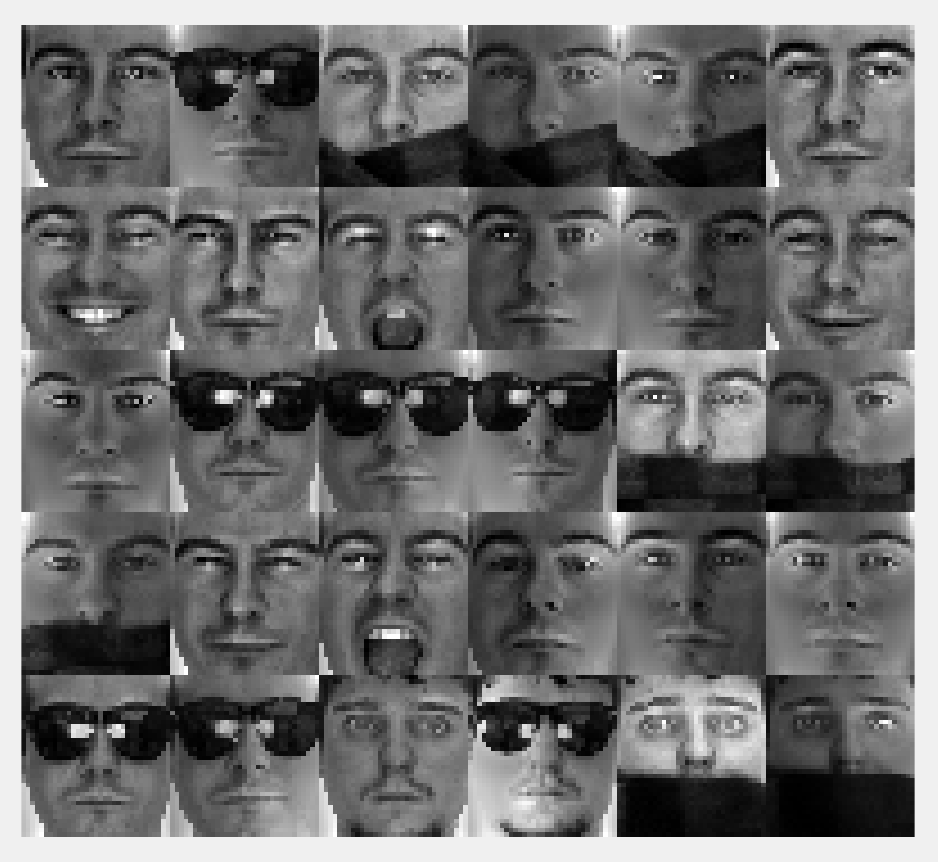
\includegraphics{img/eigenfaces}
  \caption{Eigenfaces based on PCA method}
  \label{fig:eigen}
\end{figure}


